\section{Introduction}
\label{section_intro}
In this chapter we will relate the integrated path of an asteroid to its appearance to an observer on Earth.
We will review the equatorial coordinate system, which describes the location of an object in the sky 
with the parameters right ascension (RA) and declination (DEC).
We will develop the calculations to transform between a direction from earth represented as a pair (RA, DEC)
to a direction represented as a unit vector $\uvec = (u_x, u_y, y_z)$ in the barycentric mean ecliptic frame.
We will explore the ZTF dataset of telescopic observation from the Palomar observatory in California.
We will compute the direction $\uvec$ from which an observer at Palomar would have seen an object at a given observation time
as a function of its predicted position $\qvec$ and velocity $\vvec$ at that observation time.
This calculation will account for the time required for light to reach the observatory (``light time'')
and for the location of the observatory on the surface of the earth as distinct from geocenter (``topos adjustment'').
We will run this calculation on all the known asteroids, computing the direction they would have appeared in the sky if they had been visible at Palomar.
We will use this calculation to associate each ZTF obervation with the nearest asteroid to it in the sky.

Finally, we will study the statistical distribution of angular distance between the ZTF observations and the nearest asteroid.
We will show that 65.71\% of these observations fall within 2.0 arc seconds of the direction predicted for one of the 733,489 catalogued asteroids.
We will compare this to the theoretical distribution of angular distances to the nearest asteroid 
if the predicted directions were distributed uniformly on the sphere.
We will show that such a high preponderance of ``hits'' is wildly unlikely and conclude that the asteroid catalogue 
has correct orbital elements for the objects being detected, 
and that the combined tolerance of the instruments and this calculation apparatus is on the order of 2.0 arc seconds.

\section{A Brief Review of Right Ascension (RA) and Declination (DEC)}
\label{section_ra_dec}
How can we describe the direction of an object we see in the sky?
It is a question that dates back to the first astronomers in ancient times.
The simplest and most intuitive coordinate system is the \href{https://en.wikipedia.org/wiki/Horizontal_coordinate_system}{topocentric coordinate system},
which uses the local horizon of an observer on the surface of the Earth as the fundamental plane.
In this coordinate system, an object in the sky is described in terms of an altitude (sometimes called an elevation) and an azimuth.
The altitude is how many degrees the object is above the visible horizon, so it will be between $0 \degree$ and $90 \degree$.
The topocentric coordinate system is intuitive and easy to use for an observer standing on the surface of the earth and looking at the sky.
If I wanted to do some amateur astronomy with my kids and know where to point an inexpensive telescope, these are the coordinates I would want.
\begin{figure}[hbt!]
\begin{center}
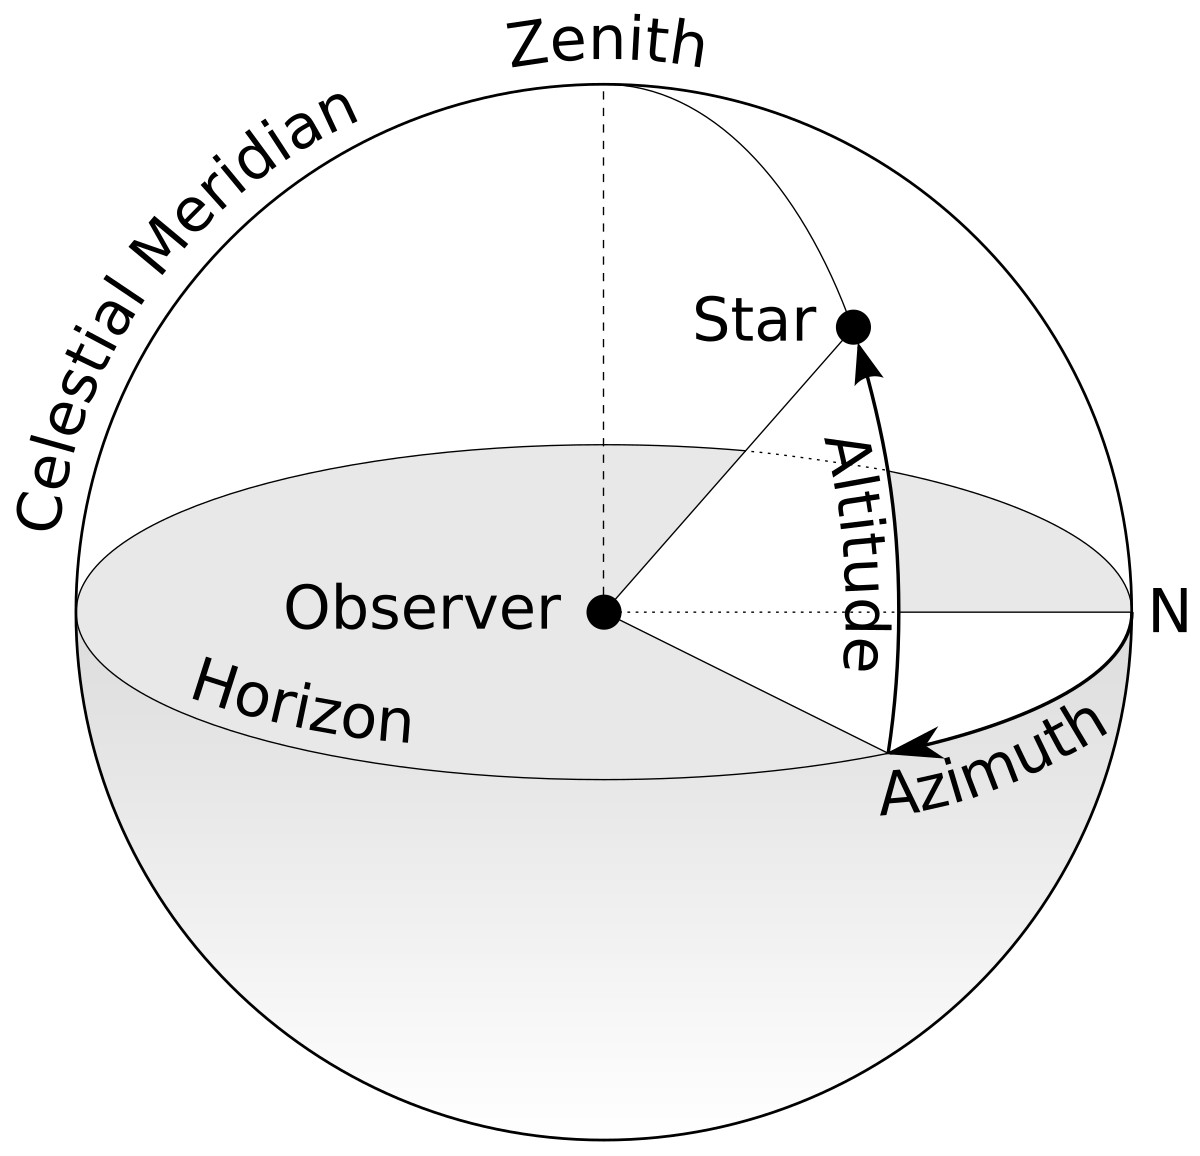
\includegraphics[width=0.6\textwidth]{topocentric_coordinates.png}
\caption{The topographic coordinate system, courtesy of \href{https://en.wikipedia.org/wiki/Horizontal_coordinate_system}{Wikipedia}}
\end{center}
\end{figure}

But the topcentric coordinate system is poorly suited to sharing observational data between astronomers.
It is a different reference frame depending on where you are located on the Earth and the time in the evening.
For this reason, astronomers dating back to ancient times developed the \href{https://en.wikipedia.org/wiki/Equatorial_coordinate_system}{equatorial coordinate system}.
This coordinate system draws an imaginary sphere around the earth.
The $x$ axis of this coordinate frame points from the Sun to the center of the Earth at the Vernal Equinox of a specific date 
(typically \href{https://en.wikipedia.org/wiki/Epoch_(astronomy)}{J2000.0} these days).
The $y$ axis is 90 degrees to the East and the $z$ axis points to the North pole.
This is much easier to understand with a picture than with words:
\begin{figure}[hbt!]
\begin{center}
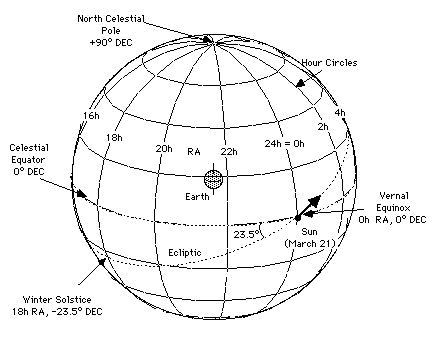
\includegraphics[width=0.8\textwidth]{celestial_sphere.png}
\caption{The celestial sphere, courtesy of \href{http://coolcosmos.ipac.caltech.edu/cosmic_classroom/cosmic_reference/coordsys.html}{cool cosmos}.}
\end{center}
\end{figure}

The celestial sphere was originally conceived as having its $z$ axis pointing along the axis of the Earth's rotation, i.e. from the South Pole to the North Pole.
This is not a good definition though for the purposes of modern astronomy, 
because the Earth's rotational axis is not a fixed direction in the barycentric mean ecliptic frame.
The Earth's rotational axis changes over time due to two separate effects: 
\href{https://en.wikipedia.org/wiki/Axial_precession}{precession} and \href{https://en.wikipedia.org/wiki/Astronomical_nutation}{nutation}.
Precession is a low frequency, predictable effect that in analagous to wobbling movement of a top's rotational axis.
It is typically covered in a first semester undergraduate physics course on mechanics.
The precession of the Earth's axis is caused by mainly by the gravitational influence of the Sun and Moon, and has a period of approximately 25,772 years.
Nutation is a high frequency effect, also caused mainly by the gravitational foreces of the Sun and Moon.
In fact, the only difference bewteen the two effects is in the way we model and understand them.
Precession isolates the mean perturbation over time; it's a slow, steady drift that is easy to predict.
Nutation describes the much smaller, high frequency wobbles (on the order of tens of arc seconds) that are the residual after precession is accounted for.

Because of the instability of the Earth's rotational axis, the definition of the directions were updated to refer to the mean ecliptic as of a date,
rather than Earth's rotational axis when the measurement is taken.
Detailed calculations of the precession and nutation can then be used to adjust measurements taken on different dates.
Ineed, the \tty{astropy} astronomy package has the capability to perform these calculations.
The diagram of the equataorial coordinate system clarifies this more modern definition.  
The vernal equinox is the moment when the Earth's orbit crosses the ecliptic.

This definition of a celestial coordinate system has in turn been superseded by a still more accurate system:
the Interational Celestial Reference System, \href{https://en.wikipedia.org/wiki/International_Celestial_Reference_System}{ICRS}.
The ICRS is based on an elegant idea.
The goal of a celestial reference frame is to provide directions that are as near to fixed as possible in the reference frame of the solar system.
Astronomers realized that since objects that are very far away from the Milky Way have orientations that are effectively fixed,
the most precise way to define directions was based on large quantities of astronomical observations of these objects.
In particular, radioastronomy (observations of stars in the radio wave frequency) is used.
This is the basis of the ICRS and the frame of reference it defines: the International Celestial Refrence Frame (ICRF).
The ICRF is a 3 dimensional coordinate system whose origin is the solar system barycenter (center of mass).
The $X$, $Y$ and $Z$ axes are set by convention to line up very closely to the traditional definition of the J2000.0 frame.
The orientation of the coordinate axes is based on the measured positions of 212 extragalactic objects, mainly quasars.
These objects are so far away from Earth and the Milky Way galaxy that they are considered ``fixed points'' in space.
\footnote{\href{http://kejian1.cmatc.cn/vod/comet/oceans/naval_observatory/navmenu.php_tab_1_page_3.2.1_type_text.htm}{U.S. Naval Observatory - ICRS}}
Modern telescopes can achieve extremely accurate RA/Dec measurements by calibrating against the measured directions to these objects.
\begin{figure}[hbt!]
\begin{center}
\includegraphics[width=0.8\textwidth]{ICRS_USNO.jpg}
\caption{The International Celestial Reference Frame (ICRF), courtesy of 
\href{http://kejian1.cmatc.cn/vod/comet/oceans/naval_observatory/navmenu.php_tab_1_page_3.2.1_type_text.htm}{U.S. Naval Observatory}.}
\end{center}
\end{figure}

The main conclusion of this short section is that even an apparently simple idea, the direction from an observer on Earth to an object seen in the sky,
is quite subtle if you want to take reproducible measurements that are accurate on the order of arc seconds.
The ICRS is accurate on the order of a handful of milliarcseconds, 
meaning that uncertainty in the coordinate frame is not a meaningful contributor to errors for any calculations in this thesis.
Fortunately this is a mature and well studied problem in astronomy, and it is addressed well by the \tty{astropy} package.
Rather than trying to reinvent the wheel, I use the \tty{astropy} as much as possible in the next section
to relate RA/Dec measurements to directions $\uvec$ in the barycentric mean ecliptic frame.

\section{Mapping Between RA/Dec and Direction $\vec{u}$ in the Ecliptic Frame}
\label{section_ra_dec_to_dir}


\section{Introducing the ZTF Dataset}
\label{section_ztf}

\section{Computing a Direction $\vec{u}$ from Position $\vec{q}$ and Velocity $\vec{v}$}
\label{section_pos_vel_to_dir}

\section{Finding the Nearest Asteroid to Each ZTF Observation}
\label{section_ztf_nearest_ast}

\section{Analyzing the Distribution of Distance to the Nearest Asteroid}
\label{section_nearest_ast_distribution}

